\documentclass[preprint]{sigplanconf}
\usepackage{amssymb}
\usepackage{amsthm}
\usepackage{graphicx}
\usepackage{amsmath}
\usepackage{mathptmx}
\usepackage{mathtools}
\usepackage{stmaryrd}
\usepackage{hyperref}
\usepackage{alltt}
\usepackage{url}
\usepackage{float}
\usepackage{tikz}
\usepackage{pgfplots}
\usepackage{style/code}
\usepackage{style/proof}
\usepackage{style/utils}
\usepackage{style/judgements}

% -----------------------------------------------------------------------------
\begin{document}

% \exclusivelicense
% \conferenceinfo{}{}
% \copyrightyear{2015}
% \copyrightdata{}
\doi{}
% \pagenumbering{gobble} 

\title{Icicle: write once, run once}

\authorinfo{
  Amos Robinson$^{\alpha \beta}$
  \and Ben Lippmeier$^{\beta \gamma}$
}{
  \vspace{5pt}
  \shortstack{
    $^\alpha$Ambiata      \\
    \textsf{amos.robinson@ambiata.com}
  }
  \shortstack{
    $^\beta$UNSW Australia\\
    ~~~~\textsf{amosr,benl@cse.unsw.edu.au}
  }
  \shortstack{
    $^\gamma$Vertigo Technology \\
    ~~\textsf{benl@vergo.co}
  }
}

\maketitle
\makeatactive

\begin{abstract}
We present Icicle, a pure streaming query language which statically guarantees that multiple queries over the same input stream will be fused. We use a modal type system to ensure that fused queries can be computed in an incremental fashion, and a fold-based intermediate language to compile down to efficient C code. We present production benchmarks demonstrating significant speedup over existing queries written in R, as well as the widely used Unix tools \texttt{grep} and \texttt{wc}.

% When querying a large amount of data, simply iterating over the data may take hours. If multiple queries are to be performed, it is important that work is not duplicated. Queries that can be performed together must be performed in the same iteration. We introduce a simple streaming language for computing queries in a single-pass over the data. With type and other restrictions we guarantee fusion between queries on the same input table, before extracting efficient C code.
\end{abstract}


%!TEX root = ../Main.tex
\section{Introduction}

Data flow fusion~\cite{lippmeier2013flow} is a technique to compile a specific class of data flow programs into single, efficient imperative loops. This process of ``compilation'' is equivalent to performing array fusion on a combinator based functional array program, as per related work on stream fusion~\cite{coutts2007streamfusion} and delayed arrays~\cite{keller2010repa}. The key benefits of data flow fusion over this prior work are: 1) it fuses programs that use branching data flows where a produced array is consumed by several consumers, and 2) complete fusion into a single loop is guaranteed for all programs that operate on the same size input data, and contain no fusion-preventing dependencies between operators.

Fusion-preventing dependencies express the fact that some operators simply must wait for others to complete before they can produce their own output. For example, in the following:
\begin{code}
  normalize :: Array Int -> Array Int
  normalize xs = let sum = fold (+) 0 xs
                 in  map (/ sum) xs
\end{code}

If we wish to divide every element of an array by the sum of all elements, then it seems we are forever destined to compute the result using at least two loops: one to determine the sum, and one to divide the elements. The evaluation of @fold@ demands all elements of its source array, and we cannot produce any elements of the result array until we know the value of @sum@. 

However, many programs \emph{do} contain opportunities for fusion, if we only knew which opportunities to take. The following example offers \emph{several} unique, but mutually exclusive approaches to fusion. Figure~\ref{f:normalize2-cluterings} on the next page shows some of the possibilities.
\begin{code}
 normalize2 :: Array Int -> Array Int
 normalize2 xs
  = let sum1 = fold   (+)  0   xs
        gts  = filter (> 0)    xs
        sum2 = fold   (+)  0   gts
        ys1  = map    (/ sum1) xs
        ys2  = map    (/ sum2) xs
    in (ys1, ys2)
\end{code}

In Figure~\ref{f:normalize2-cluterings}, the dotted lines show possible clusterings of operators. Stream fusion implicitly choses the solution on the left as its compilation process cannot fuse a produced array into multiple consumers. The best existing ILP approach will chose the solution on the right as it cannot cluster operators that consume arrays of different lengths. Our system choses the solution in the middle, which is also optimal for this example. 

% NOTE: This set of bullets needs to fit on the first page, without spilling to the second.
Our contributions are as follows:
\begin{itemize}
\item   
We extend prior work by Megiddo~\cite{megiddo1998optimal} and Darte~\cite{darte2002contraction}, with support for length changing operators. Length changing operators can be clustered with the operators that generate their source arrays, and compiled naturally with data-flow fusion (\S\ref{s:ILP}).

\item
We present a simplification to constraint generation that is also applicable to some existing integer linear programming formulations such as Megiddo's,
where constraints between two nodes need not be generated if there exists a fusion-preventing path between the two (\S\ref{s:OptimisedConstraints}).

\item
Our constraint system also encodes a total ordering on the cost of clusterings, expressed using weights on the integer linear program. For example, we encode that memory traffic is more expensive than loop overheads, so given a choice between the two, the memory traffic will be reduced (\S\ref{s:ObjectiveFunction}).

\item
We present benchmarks of our algorithm applied to several common programming patterns, and to several pathological examples.
Our algorithm is complete and yields good results in practice, though if array sizes are unknown, an optimal solution is uncomputable in general. \TODO{ref}
\end{itemize}

The reduction of the clustering problem to integer linear programming was previously described by~\cite{megiddo1998optimal}, though they do not consider length changing operators.


% We must also decide which clustering is the `best' or most optimal. One obvious criterion for this is the minimum number of loops, but there may even be multiple clusterings with the minimum number of loops. In this case, the number of required manifest arrays must also be taken into account. 

% As real programs contain tens or hundreds of individual operators, performing an exhaustive search for an optimal clustering is not feasible, and greedy algorithms tend to produce poor solutions. 


%!TEX root = ../Main.tex
\section{Icicle}
\label{s:IcicleSource}

%!TEX root = ../Main.tex

\begin{figure}

\begin{tabbing}
MMMM \= M \= MMMMMMMMMMM \= \kill
@Exp@
    \> $=$  \> $n$ \\
    \> $~|$ \> $@Prim@$ \\
    \> $~|$ \> $@Exp@~@Exp@$ \\
\\
    \> $~|$ \> $@let@~n~@=@~@Exp@$
            \> $\flowsinto~@Exp@$ \\
    \> $~|$ \> $@fold@~n~@=@~@Exp;@~@Exp@$
            \> $\flowsinto~@Exp@$ \\
\\
    \> $~|$ \> $@filter@~@Exp@$
            \> $\flowsinto~@Exp@$ \\
    \> $~|$ \> $@group@~@Exp@$
            \> $\flowsinto~@Exp@$ \\
\\
@Prim@
    \> $=$  \> $@+@~|~@>@~|~\NN~|~@scan@$ \\
\end{tabbing}


\caption{Grammar for Icicle Source}
\label{fig:source:grammar}
\end{figure}


%!TEX root = ../Main.tex

\begin{figure*}

\begin{tabbing}
MM \= MM \= \kill
$\mi{Kind}$
\GrammarDef $@Data@~|~@Clock@~|~@Flow@$ \\

T
\GrammarDef $x~|~\NN~|~\BB~|~@()@
    ~|~ @List@~T
    ~|~ @Stream@~T~T
    ~|~ @Fold@~T
    ~|~ T~\to~T$ \\
\end{tabbing}

$$
\boxed{\TypeWf{\Delta}{\tau}{\mi{Kind}}}
$$

$$
\ruleIN
{
    x~:_k~k~\in~\Delta
}
{
    \TypeWf{\Delta}{x}{k}
}{TVar}
\ruleAx
{
    \TypeWf{\Delta}{\NN}{@Data@}
}{TNat}
\ruleAx
{
    \TypeWf{\Delta}{\BB}{@Data@}
}{TBool}
\ruleAx
{
    \TypeWf{\Delta}{@()@}{@Data@}
}{TUnit}
\ruleIN
{
    \TypeWf{\Delta}{\tau}{@Data@}
}
{
    \TypeWf{\Delta}{@List@~\tau}{@Data@}
}{TList}
$$

$$
\ruleIN
{
    \TypeWf{\Delta}{c}{@Clock@}
    \quad
    \TypeWf{\Delta}{\tau}{@Data@}
}
{
    \TypeWf{\Delta}{@Stream@~c~\tau}{@Flow@}
}{TStream}
\ruleIN
{
    \TypeWf{\Delta}{\tau}{@Data@}
}
{
    \TypeWf{\Delta}{@Fold@~\tau}{@Flow@}
}{TFold}
$$

$$
\ruleIN
{
    \TypeWf{\Delta}{\tau_1}{@Data@}
    \quad
    \TypeWf{\Delta}{\tau_2}{@Data@}
}
{
    \TypeWf{\Delta}{\tau_1~\to~\tau_2}{@Data@}
}{TFunData}
\ruleIN
{
    \TypeWf{\Delta}{\tau_1}{@Flow@}
    \quad
    \TypeWf{\Delta}{\tau_2}{@Data@}
}
{
    \TypeWf{\Delta}{\tau_1~\to~\tau_2}{@Flow@}
}{TFunFlow1}
$$
$$
\ruleIN
{
    \TypeWf{\Delta}{\tau_1}{@Data@}
    \quad
    \TypeWf{\Delta}{\tau_2}{@Flow@}
}
{
    \TypeWf{\Delta}{\tau_1~\to~\tau_2}{@Flow@}
}{TFunFlow2}
\ruleIN
{
    \TypeWf{\Delta}{\tau_1}{@Flow@}
    \quad
    \TypeWf{\Delta}{\tau_2}{@Flow@}
}
{
    \TypeWf{\Delta}{\tau_1~\to~\tau_2}{@Flow@}
}{TFunFlow3}
$$



\caption{Types and their kinds}
\label{fig:source:type:kinds}
\end{figure*}


\begin{figure*}

$$
\boxed{\Typecheck{\Delta}{\Gamma}{e}{T}}
$$


$$
\ruleIN
{
    (x~:~\tau)~\in~\Gamma
}
{ 
    \Typecheck{\Delta}{\Gamma}{x}{\tau}
}{TcVar}
\ruleIN
{
    v~:~\tau
}
{ 
    \Typecheck{\Delta}{\Gamma}{v}{\tau}
}{TcValue}
\ruleIN
{
    \Typecheck{\Delta}{\Gamma}{e_1}{\tau_1~\to~\tau_2}
    \quad
    \Typecheck{\Delta}{\Gamma}{e_2}{\tau_1}
}
{ 
    \Typecheck{\Delta}{\Gamma}{e_1~e_2}{\tau_2}
}{TcApp}
$$

$$
\ruleIN
{
    \Typecheck{\Delta}{\Gamma,~x~:~\tau}{e}{\tau'}
}
{
    \Typecheck{\Delta}{\Gamma}{\lambda{}x~:~\tau.~e}{\tau~\to~\tau'}
}{TcLam}
\ruleIN
{
    \Typecheck{\Delta}{\Gamma,~x~:~\tau}{e}{\tau}
    \quad
    \TypeWf{\Delta}{\tau}{@Data@}
}
{
    \Typecheck{\Delta}{\Gamma}{@fix@~(x~:~\tau)~e}{\tau}
}{TcFix}
$$

$$
\ruleIN
{
    \Typecheck{\Delta}{\Gamma}{e_1}{@Stream@~c~\tau}
    \quad
    \Typecheck{\Delta}{\Gamma}{e_2}{@Fold@~\tau}
}
{
    \Typecheck{\Delta}{\Gamma}{@when@~e_1~e_2}{@Fold@~\tau}
}{TcWhen}
\ruleIN
{
    \Typecheck{\Delta}{\Gamma}{e_1}{@Stream@~c~@()@}
    \quad
    \Typecheck{\Delta}{\Gamma}{e_2}{@Fold@~\tau}
}
{
    \Typecheck{\Delta}{\Gamma}{@sample@~e_1~e_2}{@Stream@~c~\tau}
}{TcSample}
$$

$$
\ruleIN
{
    \Typecheck{\Delta}{\Gamma}{e_1}{\tau_1~\to~\tau_2}
    \quad
    \Typecheck{\Delta}{\Gamma}{e_2}{@Stream@~c~\tau_1}
}
{
    \Typecheck{\Delta}{\Gamma}{@mapS@~e_1~e_2}{@Stream@~c~\tau_2}
}{TcMapS}
\ruleIN
{
    \Typecheck{\Delta}{\Gamma}{e_1}{@Stream@~c~\tau_1}
    \quad
    \Typecheck{\Delta}{\Gamma}{e_2}{@Stream@~c~\tau_2}
}
{
    \Typecheck{\Delta}{\Gamma}{@zipS@~e_1~e_2}{@Stream@~c~(\tau_1,\tau_2)}
}{TcZipS}
$$

$$
\ruleIN
{
    \Typecheck{\Delta}{\Gamma}{e_1}{\tau_1~\to~\tau_2}
    \quad
    \Typecheck{\Delta}{\Gamma}{e_2}{@Fold@~\tau_1}
}
{
    \Typecheck{\Delta}{\Gamma}{@mapF@~e_1~e_2}{@Fold@~\tau_2}
}{TcMapF}
\ruleIN
{
    \Typecheck{\Delta}{\Gamma}{e_1}{@Fold@~\tau_1}
    \quad
    \Typecheck{\Delta}{\Gamma}{e_2}{@Fold@~\tau_2}
}
{
    \Typecheck{\Delta}{\Gamma}{@zipF@~e_1~e_2}{@Fold@~(\tau_1,\tau_2)}
}{TcZipF}
$$

$$
\ruleIN
{
    \Typecheck{\Delta}{\Gamma}{e_1}{\tau_1}
    \quad
    \Typecheck{\Delta}{\Gamma,~x~:~\tau_1}{e_2}{\tau_2}
}
{
    \Typecheck{\Delta}{\Gamma}{@let@~x~=~e_1~@in@~e_2}{\tau_2}
}{TcLet}
$$

$$
\ruleIN
{
    \Gamma'~=~\Gamma,~\{~x_i~:~@Fold@~\tau_i~\}_i
    \quad
    \{
    \Typecheck{\Delta}{\Gamma}{e_{z_i}}{\tau_i}
    \}_i
    \quad
    \{
    \Typecheck{\Delta}{\Gamma'}{e_{k_i}}{@Fold@~\tau_i}
    \}_i
    \quad
    \Typecheck{\Delta}{\Gamma'}{e}{\tau}
}
{
    \Typecheck{\Delta}{\Gamma}
        {@let@~@folds@~\{~x_i~=~e_{z_i}~@then@~e_{k_i}~\}_i~@in@~e}
        {\tau}
}{TcLetFolds}
$$

$$
\ruleIN
{
    \Typecheck{\Delta}{\Gamma}{e_1}{@Fold@~\tau_1}
    \quad
    x_\tau~\not\in~\Delta
    \quad
    \Typecheck
        {\Delta,~x_\tau :_k @Data@}
        {\Gamma,~x_z : x_\tau,~x_k : @Fold@~x_\tau \to @Fold@~x_\tau,~x_r : @Fold@~x_\tau \to @Fold@~\tau_1}
        {e_2}{\tau_2}
}
{
    \Typecheck{\Delta}{\Gamma}
        {@let@~@unpack@~(x_\tau,x_z,x_k,x_r)~=~e_1~@in@~e_2}
        {\tau_2}
}{TcLetUnpack}
$$

$$
\ruleIN
{
    \Typecheck{\Delta}{\Gamma}{e_1}{@Stream@~c~\BB}
    \quad
    x_c~\not\in~\Delta
    \quad
    \Typecheck
        {\Delta,~x_c :_k @Clock@}
        {\Gamma,~x_s : @Stream@~x_c~\BB}
        {e_2}
        {\tau_2}
}
{
    \Typecheck{\Delta}{\Gamma}
        {@let@~@subrate@~(x_c,x_s)~=~e_1~@in@~e_2}
        {\tau_2}
}{TcLetSubrate}
$$


\caption{Types of expressions}
\label{fig:source:type:exp}
\end{figure*}


%!TEX root = ../Main.tex

\begin{figure*}

\begin{tabbing}
MMM \= MM \= MMM \= MM \= MMMMMM \= \kill
$\mi{V}$
\GrammarDef
  $\NN~|~\BB~|~@Map@~(V \Rightarrow V_\bot)~|~(V~\times~\cdots~\times~V)$
\\
$\mi{V'}$
\GrammarDef
  $\VValue{V}~|~\VStream{(\Sigma \to V)}~|~\VFold{V}{(\Sigma \to V \to V)}{(V \to V)}$
\\
$\mi{E'}$
\GrammarDef
  $\mi{Exp}[V~:=~V']$
\\
\end{tabbing}

$$
\boxed{\SourceStepX{E'}{V'}}
$$

$$
\ruleIN
{
    v~\in~V'
}
{
    \SourceStepX{v}{v}
}{EVal}
\ruleIN
{
    \SourceStepX{e}{\VValue{v}}
}
{
    \SourceStepX{e}{\VStream{(\lam{\sigma} v)}}
}{EBoxStream}
\ruleIN
{
    \SourceStepX{e}{\VValue{v}}
}
{
    \SourceStepX{e}{\VFold{()}{(\lam{\sigma~()} ())}{(\lam{()} v)}}
}{EBoxFold}
$$

$$
\ruleIN
{
  \{ \SourceStepX{e_i}{\VValue{v_i}} \}_i
}
{
  \SourceStepX
    {p~\{ e_i \}_i }
    {\VValue{(p~\{v_i\}_i)}}
}{EPrimValue}
\ruleIN
{
  \{ \SourceStepX{e_i}{\VStream{v_i}} \}_i
}
{
  \SourceStepX
    {p~\{ e_i \}_i }
    {\VStream{(\lam{\sigma} p~\{v_i~\sigma\}_i)}}
}{EPrimStream}
$$

$$
\ruleIN
{
  \{ \SourceStepX{e_i}{\VFold{z_i}{k_i}{x_i}} \}_i
}
{
  \SourceStepX
    {p~\{ e_i \}_i }
    {\VFold
      {(\times_i~z_i)}
      {(\lam{\sigma~(\times_i~v_i)}
        \times_i (k_i~\sigma~v_i))}
      {(\lam{(\times_i~v_i)}
        p~\{x_i~v_i\}_i)}}
}{EPrimFold}
$$

$$
\ruleIN
{
  \SourceStepX{e}{v}
  \quad
  \SourceStepX{e'[x:=v]}{v'}
}
{
  \SourceStepX
    {@let@~x~=~e~@in@~e'}
    {v'}
}{ELet}
\ruleIN
{
  \SourceStepX{z}{\VValue{z'}}
  \quad
  \SourceStepX{k[x:=\VStream{(\lam{\sigma} \sigma~x)}]}{\VStream{k'}}
}
{
  \SourceStepX
    {@fold@~x~=~z~@then@~k}
    {\VFold
      {z'}
      {(\lam{\sigma~v} k'~(x:=v,~\sigma))}
      {(\lam{v} v)}}
}{EFold}
$$

$$
\ruleIN
{
  \SourceStepX{p}{\VStream{p'}}
  \quad
  \SourceStepX{e}{\VFold{z}{k}{x}}
}
{
  \SourceStepX
    {@filter@~p~@of@~e}
    {\VFold
      {z}
      {(\lam{\sigma~v}
         @if@~p'~\sigma~@then@~k~\sigma~v~@else@~v)}
      {x}}
}{EFilter}
$$

$$
\ruleIN
{
  \SourceStepX{p}{\VStream{p'}}
  \quad
  \SourceStepX{e}{\VFold{z}{k}{x}}
}
{
  \SourceStepX
    {@group@~p~@of@~e}
    {\VFold
      {\{\_~\Rightarrow~\bot\}}
      {(\lam{\sigma~m}
        @let@~k~=~p'~\sigma@,@~
              v~=~m~k~\vee~z
        ~@in@~
          m[k~\Rightarrow~k~\sigma~v])}
      {\{k_i~\Rightarrow~x~(m~k_i)\}_i}}
}{EGroup}
$$


\caption{Evaluation rules}
\label{fig:source:eval}
\end{figure*}




The grammar for Icicle is given in figure~\ref{fig:source:grammar}.
Value types are given in $T$ and can be numbers, booleans or maps.
Modal types, $T_M$ can be a pure value type, or a modality associated with a value type.
Function types, $T_\to$, can be either a non-function modal type, or a function from modal type to function type.
As Icicle is a first-order language, function types are not value types.

The table definition in $\mi{Table}$ gives a table name and the names and types of columns.
$\mi{Exp}$ defines the expressions used as query and function bodies.
$\mi{Prim}$ defines the primitive types.
Function definitions are given in $\mi{Fun}$.
Query definitions are given in $\mi{Query}$.
$\mi{Top}$ is the top-level program, which specifies a table, the set of function bindings, and the set of queries.

\TODO{update this to fit new grammar}
Expressions can be variable names, primitive operators such as addition and division, function application, or nested queries.
Function application @x Exp*@ is the name of a top-level function applied to any number of arguments.
Primitive application @Prim Exp*@ is written prefix, but in the following we use infix-operator short-hand for convenience; for example, @(>) 0 1@ can be written as @0 > 1@.

Queries can define folds over the input, let-bindings, filtering according to some predicate, or grouping by some key.
The fold form takes the name of the fold binding, and two expressions: the initial value and the update value for each element.
Count can be expressed by the following fold:
\begin{code}
fold count = 0 then count + 1
\end{code}

Let-bindings allow a name to be used in place of the expression, in the rest of some query.
\begin{code}
let diff = open - close
in  mean diff
\end{code}

Filters take a predicate, which can be thought of as a stream of booleans, and a query to perform for the satisfying values.
The following query will count the number of entries where the open price exceeds the close price.
\begin{code}
filter open > close in count
\end{code}

Filters correspond to @WHERE@ clauses in SQL, except that the predicate does not apply to the entire top-level query, only to the subquery.
This makes it slightly easier to define queries like the proportion of entities satisfying some predicate to all entities: 
\begin{code}
(filter open > close in count) / count
\end{code}

Group takes a key to group by, and a query to perform on the values of each grouping.
This query groups by the company code, and counts the number of records in each company.
\begin{code}
group company in count
\end{code}

@Fun@ is used for function definitions.
The @count@ function takes no arguments and returns a fold counting the number of elements.
\begin{code}
function count
 = fold c = 0 then c + 1
\end{code}

Sum can be defined taking a single argument, @value@, which is the elements to compute the sum of.
It returns a fold that starts at zero and for every element, increases the old sum by @value@.
\begin{code}
function sum (value : Element Int)
 = fold s = 0 then s + value
\end{code}

The definition of mean is just the sum divided by the count.
\begin{code}
function mean (value : Element Int)
 = sum value / count
\end{code}




\subsection{Single-pass restriction}

All Icicle queries must execute in a single pass over the data, as reading the data multiple times is expensive. 
Ensuring that queries only require a single pass over the data also allows us to resume queries from where they left off, when new data arrives.

In order to ensure that queries can be executed as a single pass, we use a modal type system inspired by staged computation\cite{davies2001modal}.
We introduce two modalities, called @Element@ and @Aggregate@, which denote when computations must occur.

The @Element@ modality means that a computation is defined for each record in the table, or element in the stream.
Each column in the table is @Element@; for example the @open@ column has type @Element Int@, meaning that for each record in the column there is an @Int@.
This can be thought of as being represented by a stream of values.

The @Aggregate@ modality means that a computation is available only after all records in the table have been seen, or after the end of the stream.
These are used for the results of folds.
When computing count, the final value is not known until all the records have been seen, so @count@ has type @Aggregate Int@.

The modalities are automatically boxed and unboxed, so that if a function expecting a pure value is passed an @Element@ computation, the result of the function becomes an @Element@ computation too.
For example, if @open : Element Int@, then @open == 1@ has type @Element Bool@.
@Element@ and @Aggregate@ are mutually exclusive: a computation cannot be both an element and an aggregate.

Some examples with their types:
\begin{code}
1             :         Int
open          : Element Int
open > 1      : Element Int
sum           : Element Int -> Aggregate Int
sum open      : Aggregate Int
sum open > 1  : Aggregate Bool
\end{code}

Folds have a name and two expressions.
The first expression, the initialiser, is pure.
The second expression, the update, has the fold's name bound to an @Element@ of the previous value.
The type of the expression must be @Element@.
The final return of the fold is an @Aggregate@.
\begin{code}
fold x = T then Element T : Aggregate T
\end{code}

Let-bindings are independent of the modality.

For filters, the predicate is an @Element@, which could be thought of as a stream of booleans.
The rest of the query must be an @Aggregate@; that is, it must return a scalar rather than a stream, to enforce the bounded buffer restriction explained in \sref{s:IcicleSource:bounded}.
\begin{code}
filter (Element Bool) in (Aggregate T)
\end{code}

Grouping is similar to filters; the key must be an @Element@, while the group value must be an @Aggregate@.
\begin{code}
group (Element Key) in (Aggregate Value)
\end{code}

The following program attemps to find the number of entries where the open price is above the mean of the close price.
This requires two passes over the data, as we do not know what the mean of all the data is until we have seen all the data.
This program violates the single-pass restriction, and is outlawed by the typesystem.
The left side of the @>@ has type @Element Int@, while the right side has type @Aggregate Int@, and these two are mutually exclusive.
\begin{code}
filter open > mean close
in count
(Error: (>) must be Element and Aggregate)
\end{code}



Here is an example to highlight one benefit of tracking these modalities.
Suppose we have a table with two fields: key and value.
We wish to find the mean of values whose key matches the most recent key.
Someone new to stream programming might write the following query, forgetting that they can only read the data once: first find the most recent key, then go back and filter all the data to only thosewith the right key.

\begin{code}
   let k    = newest key
in let avg  = filter (key == k) in mean value
in avg
\end{code}

This will not typecheck in Icicle, as @newest key@ has the modality @Aggregate@, while the filter condition @key == k@ attempts to check if an @Element@ is equal to an @Aggregate@.

This query could be translated to another synchronous streaming language such as {\sc Lustre}\cite{halbwachs1991synchronous}, and would typecheck.
However, the semantics of the translated query will not be what was originally desired.
Rather than checking each key against the most recent key as-of the end of the stream,
it will check each key against the current most recent key, which is the key itself.
This means the filter predicate is always be true, and thus returns the mean of the entire stream.
These semantics may be surprising to the novice stream programmer.

Hopefully our programmer is not too discouraged by the @Element /= Aggregate@ type error, and pushes on.
They now know that their query, as formulated, requires multiple passes over the data: the problem now is to reformulate it as a single pass.
With a little ingenuity, we can rewrite it as such: we can group by the key and perform the mean for each group.
After the group, we can perform a lookup by the most recent key.
This requires storing and computing the means for all keys despite only needing one at the end, so we are assuming that the number of keys are bounded in some way.

\begin{code}
   let k    = newest key
in let avgs = group  key in mean value
in mapLookup avgs k
\end{code}

\subsection{Bounded buffer restriction}
\label{s:IcicleSource:bounded}
As Icicle is designed to be a streaming language, the amount of data to be streamed may not necessarily fit in memory.
Any operation which requires a buffer must be bounded in size, as an unbounded buffer could potentially grow too large to fit in memory.

Here is an example stream program that requires unbounded buffering:
it takes an input stream @xs@, and filters it into those above zero, and those below zero.
These two filtered streams are then joined together pairwise, so the first positive element is paired with the first negative element, and so on.
The program, written in Haskell:

\begin{code}
zip (filter (>0) xs) (filter (<0) xs)
\end{code}

This program requires an unbounded buffer: if the input stream contains ten positive values followed by one negative value, all ten of the positive values must be held onto until the negative value is seen.
Similarly, if the entire stream is positive, all of the elements must be retained until the very end, just in case a negative value shows up.

In Icicle, we outlaw this kind of program by implicitly threading the input stream through operations.
The streams themselves are not materialised in the program: stream operations like @fold@ and @filter@ do not take parameters of the streams, but instead operate on the context stream.
By removing the explicit stream parameter, stream elements can only be joined from the same context, when both elements are available.

For example, in the query @filter p in mean value@, the @mean value@ is only applied to stream values which satisfy the predicate @p@.

This is a different approach than existing synchronous streaming languages\cite{mandel2010lucy} and flow fusion\cite{lippmeier2013data}, which perform clock analysis or `rate inference'.
Here, streams are given clock types denoting when the streams have elements available, and only streams with the same clock can be zipped together.
Filters produce a stream with a different output clock to its input, so different filters cannot be zipped together.
Our system requires no clock analysis, but is less expressive as streams are not `first class'.


%!TEX root = ../Main.tex
\clearpage
\section{Intermediate language}
\label{s:IcicleCore}
\TODO{PAGE LAYOUT REMOVE CLEARPAGE}

\begin{figure}

\begin{tabbing}
MMM \= MM \= MMMM \= MM \= MMMMMM \= \kill
$\mi{PlanX}$
\GrammarDef
  $x~|~V~|~\mi{PlanP}~\ov{\mi{PlanX}}~|~\lam{x}\mi{PlanX}$
\\
$\mi{PlanP}$
\GrammarDef
  $\mi{Prim}~|~@mapUpdate@~|~@mapEmpty@~|~@mapMap@~|~@mapZip@$
\\
\\
$\mi{Plan}$
\GrammarDef
  $@plan@~x$ \> $\{~\ov{x~:~T;}~\}$
\\
  \> \> $@before@$ \> $\{~\ov{x~:~T~=~\mi{PlanX};}~\}$ \\
  \> \> $@folds@$  \> $\{~\ov{x~:~T~=~\mi{PlanX}~@then@~\mi{PlanX};}~\}$ \\
  \> \> $@after@$  \> $\{~\ov{x~:~T~=~\mi{PlanX};}~\}$ \\
  \> \> $@return@$ \> $\{~\ov{x~:~T~=~x;}~\}$ \\
\end{tabbing}



\caption{Query Plan Grammar}
\label{fig:core:grammar}
\end{figure}

The intermediate language can be thought of as similar to a query plan in other databases.
Queries in the source language are converted to query plans, and then query plans on the same table are fused together.
Common subexpression elimination, partial evaluation and other optimisations are performed at the query plan level.

The grammar for the intermediate language is given in figure~\ref{fig:core:grammar}.
Expressions can be variables, values, applications of primitives or anonymous functions.
Function definitions and uses are not allowed in expressions here, as their definitions are inlined before converting to query plans.
Anonymous functions are only allowed as arguments to primitives: they cannot be applied or stored in variables.
The $\mi{Plan}$ itself is split into stages of computation, which correspond to the modal stages in the Source query.
The first stage, @before@, is used for pure computations which do not depend on any stream values at all.
The next stage, @folds@, defines the @Element@ computations and how they are converted into @Aggregate@ computations.
Next are @after@ which correspond to @Aggregate@ computations, occurring after the entire stream has been seen.
Finally, the @return@ specifies the output values of the query; a single query will have only one output value, but the result of fusion can have many outputs.

We will start with a small example by converting just the @last key@ part of the group-mean query.
Here, we have the function definition for @last k@, which is defined as a fold with an initial value to describe a missing date @NO_DATE@, and the update value is the current @k@.
The current fold value is bound to @l@ but is not used.

\begin{code}
    table kvs { key : Date; value : Real } 

    function last (d : Element Date)
     = fold l = NO_DATE then d;

    query last_key = last key
\end{code}

We now inline function definitions before converting to a query plan, renaming as necessary.
This is guaranteed to terminate because no recursion is allowed in function definitions.

\begin{code}
==> table kvs { key : Date; value : Real } 
    query last_key = (fold c = NO_DATE then key)
\end{code}

We can now convert this to a query plan.

\begin{code}
==> plan kvs { key : Date; value : Real; }
    before { }
    folds  { c : Date = NO_DATE then key }
    after  { }
    return { last_key : Date = c }
\end{code}

We will now convert the mean group.
Here, we have function definitions for @count@, @sum@ and @mean@.
Count is defined by starting from zero, and incrementing by one for each element.
Sum starts at zero and increments its argument.
Mean is then defined as sum divided by the count.

\begin{code}
    table kvs { key : Date; value : Real } 

    function count
     = fold c = 0 then c + 1;

    function sum (e : Element Real)
     = fold s = 0 then s + e;

    function mean (e : Element Real)
     = sum e / count;

    query mean_all = group key of mean value
\end{code}

After function inlining, the result is this:
\begin{code}
==> table kvs { key : Date; value : Real } 
    query mean_all = group key
     of (fold foldS = 0 then foldS + value)
      / (fold foldC = 0 then foldC + 1)
\end{code}

Finally, we have the query plan.
Each fold inside the group becomes its own map which is initialised to empty.
At each iteration the fold update is applied to the value in the map, or the fold's initial value if the key is not yet present.
After all iterations are finished, the two maps are joined together and the pairs are divided.
\begin{code}
==> plan kvs { key : Date; value : Real; }

    before { }

    folds  { groupS   : Map Date Real
                = mapEmpty
             then mapUpdate groupS key 0
                  (\foldS. foldS + value)

           ; groupC   : Map Date Real
                = mapEmpty
             then mapUpdate groupC key 0
                  (\foldC. foldC + 1) }

    after  { groupM   : Map Date Real
                = mapMap (/) (mapZip groupS groupC) }

    return { mean_all : Map Date Real = groupM }
\end{code}

It is possible to convert this as a map of pairs of the sum and count.
Keeping this as two separate maps rather than a map of pairs exposes more opportunities for common subexpression elimination when fusion occurs.
For example, a query @group key of count@ can reuse the already constructed @groupC@ map.


If we now wish to fuse these query plans together, it is as simple as giving the bindings unique names, and appending each part of the plan together.
The names of the returns and the column names stay the same.
Query plans can only be fused if they act on the same table.

The above query plan computes all three queries at once, but has some duplicate work: the counts and the sums are performed twice.
We can perform common subexpression elimination to remove these.

The interesting thing here is just how simple fusion is.
Thanks to the single-pass restriction, we know there are no dependencies between any two query plans: if there were, the source query would have required multiple passes.
The single-pass restriction means that any source query can be expressed as a single fold over the data.

An efficient imperative loop can be generated from this query plan rather easily, in a similar way as previous work on flow fusion~\cite{lippmeier2013data}.


%!TEX root = ../Main.tex
\section{Benchmarks}
\label{s:Benchmarks}
%!TEX root = ../Main.tex

\begin{figure}

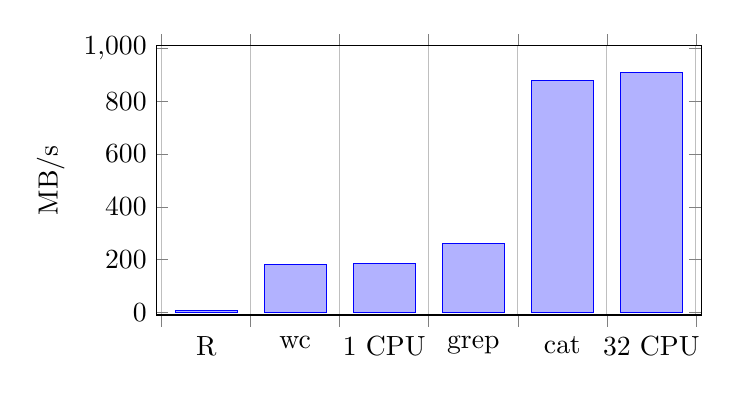
\begin{tikzpicture}
\begin{axis}[
	ylabel=MB/s,
  ymin=0, ymax=1000,
	enlargelimits=0.01,
	ybar interval=0.7,
  symbolic x coords={R, wc, 1 CPU, grep, cat, 32 CPU, end},
  width=8.5cm, height=5cm,
]
\addplot coordinates {(R,6.0) (wc,182.6) (1 CPU,186.6) (grep,261) (cat,878) (32 CPU,908) (end,0) };
% \addplot coordinates {(R,6.0) (wc,182.6) (CPU1,186.6) (grep,261) (wc -l,852) (cat,878) (Run 372,908) (Run 1,1029) (end,0) };

% \legend{MB/s}

\end{axis}
\end{tikzpicture}

\caption{Throughput comparisons of Icicle (1 CPU and 32 CPU) against existing R code and standard Unix utilities; higher is faster.}
\label{fig:bench:other}
\end{figure}



At Ambiata, we are currently using Icicle in production over medium-sized datasets that fit on a single disk.
These initial results have been very promising, and we are currently implementing distribution across multiple machines to handle datasets that are tens of terabytes compressed, and do not fit on a single disk.
Incremental computation is even more important for this distributed case, as we can avoid copying terabytes of data over the network.

We evaluated Icicle by replacing an R script which ran weekly in production.
This R script works over around three hundred gigabytes of PSV data.
It computes twelve queries over each of the thirty-one input tables, computing 372 queries in total.

The R script for this takes fifteen hours to run and is 3,566 lines of code.
In contrast, our Icicle queries take seven minutes to run, and the dictionary describing the queries is 191 lines of code.

The table in figure~\ref{fig:bench:other} shows the throughput in megabytes per second.
We compared the throughput of several programs over the same 317GB dataset:
\begin{itemize}
\item our original R implementation (R);
\item Icicle running single-threaded (1 CPU);
\item Icicle running on multiple processors (32 CPU);
\item finding empty lines with @grep "^$"@;
\item counting characters, words and lines with @wc@;
\item reading and throwing away the results with @cat > /dev/null@.
\end{itemize}

We ran all of the Unix utilities with unicode disabled using @LANG=C LC_COLLATE@ for maximum performance.
The computer we used for most of these was an Amazon EC2 @c3.8xlarge@ with 32 CPUs, 60GB of RAM, and striped, RAIDed SSD storage.
The R code requires an @i2.8xlarge@ with 244GB of memory, but we were unable to perform our other benchmarks on such a large machine.
Icicle significantly outperformed R, and the single-threaded version was on par with @wc@, while only a little slower than @grep@.
This is despite doing conceptually more work than @wc@ and @grep@.
By using multiple processors, we were able to scale up to perform as well as @cat@, approaching the disk speed.
The R code is single threaded and would require at least 150 processors to reach similar speeds, assuming perfect scaling.
These results give us confidence that our distributed implementation will be fast as well as scalable~\cite{mcsherry2015scalability}.

%!TEX root = ../Main.tex

\begin{figure}

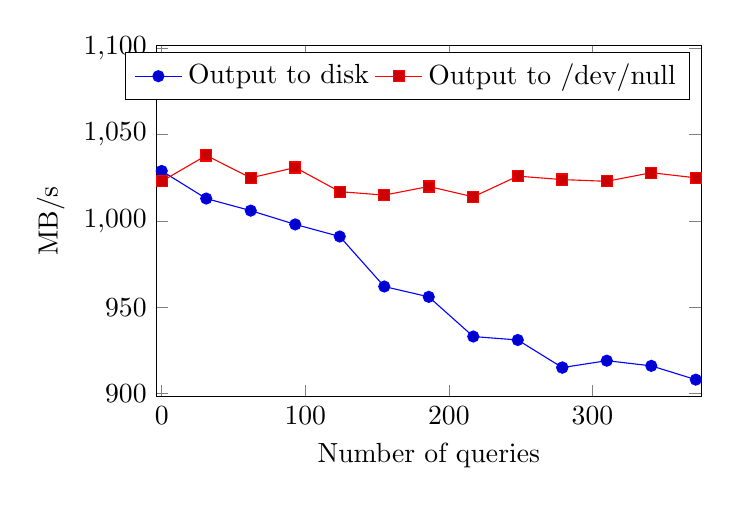
\begin{tikzpicture}
\begin{axis}[
	x tick label style={/pgf/number format/1000 sep=},
	ylabel=MB/s,
  ymin=900, ymax=1100,
%  xmax=372,
  xlabel=Number of queries,
	enlargelimits=0.01,
	legend style={legend columns=-1},
  width=8.5cm, height=6.05cm,
%	legend style={at={(0.5,-0.1)},anchor=north,legend columns=-1},
%	ybar interval=0.7,
]

% bench/raw.txt
% Running with fewer queries
% \addplot coordinates {(0,1025.5) (1,1029.6) (48,978) (96,941) (144,943) (192,936) (240,904) (276,895.5) (324,881) (372,846.2) };

% bench/raw.txt
% Running with fewer queries, better distribution
% \addplot coordinates { (0,1029) (31,1013) (62,1006) (93,998) (124,991) (155,941) (186,956) (217,933) (248,931) (279,915) (279,915) (310,919) (341,916) (372,908) };

%% APPLY LOPASS
\addplot coordinates { (0,1029) (31,1013) (62,1006) (93,998) (124,991) (155,962) (186,956) (217,933) (248,931) (279,915) (279,915) (310,919) (341,916) (372,908) };


% Fusion, no output
% \addplot coordinates { (0,1001) (31,1038) (62,1025) (93,1031) (124,1006) (155,1015) (186,1020) (217,997) (248,1026) (279,1024) (310,1009) (341,1038) (372,1025) };

%% APPLY LOPASS
\addplot coordinates { (0,1023) (31,1038) (62,1025) (93,1031) (124,1017) (155,1015) (186,1020) (217,1014) (248,1026) (279,1024) (310,1023) (341,1028) (372,1025) };

% No fusion, no output
% \addplot coordinates { (0,987) (31,1037) (62,1024) (93,1002) (124,1037) (155,1024) (186,1004) (217,1040) (248,1023) (279,998) (310,1018) (341,1013) (372,1003) };

\legend{Output to disk, Output to /dev/null};

\end{axis}
\end{tikzpicture}


\caption{Decrease in read throughput as queries are added, comparing writing the output to disk and writing to /dev/null.}
\label{fig:bench:queries}
\end{figure}


% \begin{figure}
% \begin{tikzpicture}
% \begin{axis}[
% 	x tick label style={/pgf/number format/1000 sep=},
% 	ylabel=MB/s,
%   ymin=0, ymax=1200,
%   xlabel=Number of threads,
% 	enlargelimits=0.01,
% 	legend style={legend columns=-1},
% ]
% \addplot coordinates { (1,163) (2,335) (3,442) (4,532) (5,578) (6,615) (7,633) (8,628) (9,631) (10,626) (11,637) (12,643) (13,658) (14,795) (15,781) (16,798) (17,840) (18,864) (19,862) (20,867) (21,847) (22,877) (23,876) (24,884) (25,862) };
% \end{axis}
% \end{tikzpicture}
% \caption{Scaling as threads are added}
% \label{fig:bench:scaling}
% \end{figure}




Figure~\ref{fig:bench:queries} shows how Icicle scales in throughput as more queries are added.
We ran two versions with each number of queries; one version writing output to disk, and the other throwing away the result to @/dev/null@ rather than spending time writing.
The graph shows the disk version decreasing roughly linearly in the number of queries, while the version ignoring the output stays constant.
This suggests that the output code is the bottleneck, which is unsurprising given the output format is text-based PSV.
The upshot of this is that the time spent computing the queries appears constant as hundreds of queries are added, which suggests that many more queries can be handled if a better output format is used.


% %!TEX root = ../Main.tex
\section{Conclusion}
\label{s:Conclusion}

By designing a restricted language, we have a language which is just expressive enough to be useful, while retaining important performance guarantees.



% %!TEX root = ../Main.tex
\section{Elimination}
\label{s:Elimination}


Horizontal fusion for imperative loops is relatively easily, when the loops have the same number of iterations.
The problem with imperative loops occurs when trying to remove duplicate computations.
Firstly, the `definition' of a computation is split across multiple places: because the initial value of an accumulator and its update expression are in separate parts of the program, some analysis must be done to recover these.
For example, in the following loop, @a@ and @b@ have equivalent `update' expressions, but could denote very different computations depending on the implementation of @function@.
\begin{code}
a = 0;
b = 1;
for (...) {
  a = function(a);
  b = function(b);
}
\end{code}

Secondly, the order of statements in a loop affects the meaning: when accumulators are mutually dependent on each other, one can reorder the statements to produce a different, but still valid program.
These two loops are not equivalent:
\begin{code}
a = 0;
b = 1;
for (...) {
  a = a + b;
  b = a - b;
}
for (...) {
  b = a - b;
  a = a + b;
}
\end{code}

Neither of these problems are insurmountable, but the analysis required certainly complicates our goal of removing duplicate computation after fusion.

With this in mind, we will introduce our intermediate language based on what we call ``fold nests'', as opposed to loop nests.
Firstly, each accumulator should be defined in one place: this means that if two accumulators are alpha equivalent, they are equivalent.
Secondly, reordering statements (or accumulators) should not affect the meaning: two programs are equivalent if they contain equivalent sets of bindings, regardless of ordering.

We now convert the first example to folds:
\begin{code}
a = 0;
b = 1;
for (...) {
  a = function(a);
  b = function(b);
}

==>
loop ... {
  stage {
    fold a = 0
        then function(a);
  }
  stage {
    fold b = 1
        then function(b);
  }
}
\end{code}

Each fold binding must be grouped inside a @stage@ block, which allows mutual recursion across folds.
In this case, there is no mutual recursion, so the stages only contain one binding each.
The first fold is given the name @a@ with @fold a@.
Its initial value comes straight after the equals sign, so @a@ starts with a value of @0@.
The update or `kons' expression comes after @then@, and in the update expression any reference to @a@ refers to the current value of the fold.

It now becomes easier to see that the two folds are not equivalent, as the entire definitions are in one place.

The next example requires mutual recursion.
\begin{code}
a = 0;
b = 1;
for (...) {
  a = a + b;
  b = a - b;
}

==>
loop ... {
  stage {
    fold a = 0
        then a + b;
    fold b = 1
        then new a - b;
  }
}
\end{code}

Here, the update expression for @a@ refers to a later fold, @b@.
Update expressions can refer to later fold bindings in the same stage, as well as all earlier fold bindings.
The value referred to is the value of the binding at the start of the iteration, before any updates have occurred.
The new value of earlier folds, after being updated, can be referred to by suffixing a prime to the name: in the binding for @b@, the updated @a@ is referred to by @new a@.
This restriction of only accessing the new value of earlier folds is akin to the causality restriction in dataflow languages\cite{mandel2010lucy}.

Another way to think of the new value restriction above is disallowing cycles in the references to new values:
when @b@ references @new a@, the new value of @a@, it means that @new a@ must be computed before @new b@ can be.
If there were a cycle where @new a@ also depended upon @new b@, there would be no order to compute them in.
Disallowing cycles ensures an execution order.

By making the distinction between `old value' and `new value' explicit, the ordering in the program no longer has any effect on the semantics.
After converting the reordered loop with different semantics, the two programs are no longer alpha-equivalent:
\begin{code}
a = 0;
b = 1;
for (...) {
  b = a - b;
  a = a + b;
}

==>
loop ... {
  stage {
    fold b = 1
        then a - b;
    fold a = 0
        then a + new b;
  }
}
\end{code}

\subsection{Preliminary transforms}

A-normalisation is relatively easy, however any expressions in the initialiser of each fold can be lifted out as a separate fold with initialiser and an identity expression (that is, the name of the fold).
Any expressions to be lifted out from the update expression should be created as new @let@ bindings.
They cannot necessarily be created as @fold@ bindings because the expression will not work for the initial expression, if it refers to other lets or loop iterators.

Some simple forwarding can be applied, such as lets of variables, and folds where the initial and update expressions are the same.
Fold initials could be forwarded to other initials, but fold updates cannot always be forwarded to other updates, as the first evaluation of the other update will refer to the forwarder's initial.

So-called ``melting'' can be performed, splitting apart pairs into multiple bindings, arrays of pairs into pairs of arrays, and so on.
Key-value maps can be similarly split into a special map from key to index, and an array for the values.
Splitting these complex structures into their constituent parts exposes more opportunities for elimination removal.
The following program computes the mean of the loop elements. Here, the sum and count are both computed, and stored in a pair.

\begin{code}
loop item {
  stage {
    fold sumcount
     = (0, 0)
     then
       ( fst sumcount + item
       , snd sumcount + 1);

    fold mean
     = fst sumcount / snd sumcount
     then
       fst sumcount / snd sumcount;
  }
}
\end{code}

If another query were to compute the sum as well, it is not obvious looking at the two expressions that @sum@ and @fst sumcount@ are equivalent:
\begin{code}
loop item {
  stage {
    fold sum
     = 0
     then
       sum + item;
  }
}
\end{code}

Now, by splitting the @sumcount@ pair into two bindings named @sumcount1@ and @sumcount2@, it becomes easier to see that the definitions of @sum@ and @sumcount1@ are equivalent.
\begin{code}
loop item {
  stage {
    fold sumcount1
     = 0
     then
       sumcount1 + item;

    fold sumcount2
     = 0
     then
       sumcount2 + 1;

    fold mean
     = sumcount1 / sumcount2
     then
       sumcount1 / sumcount2;
  }
}
\end{code}


\subsection{Stage-local duplicate removal}
Here is an example of a stage with two counters.
\begin{code}
stage {
  fold a = 0 then c + 1
  fold b = 0 then c + 1
  fold c = 0 then a + b
}
Execution:
[ a = 0, b = 0, c = 0 ]
[ a = 1, b = 1, c = 0 ]
[ a = 1, b = 1, c = 2 ]
[ a = 3, b = 3, c = 2 ]
[ a = 3, b = 3, c = 6 ]
[ a = 7, b = 7, c = 6 ]
[ a = 7, b = 7, c = 14 ]
\end{code}

The bindings for @a@ and @b@ here are identical, and so one can be replaced with the other, by substituting @b := a@ and removing the binding for @b@.
\begin{code}
stage {
  fold a = 0 then c + 1
  fold c = 0 then a + a
}
\end{code}

Another example is a single count, spread across two recursive bindings.
Here, @a@ and @b@ depend on each other, but both have the same body modulo alpha.
\begin{code}
stage {
  fold a = 0 then b + 1
  fold b = 0 then a + 1
}
Execution:
[ a = 0, b = 0 ]
[ a = 1, b = 1 ]
[ a = 2, b = 2 ]
\end{code}

One can place them into equivalence groups based on their bodies: @a@ and @b@ go in the same equivalence group, and so any reference to @a@ or @b@ refers to the equivalence group containing both.
Equivalence groups are then squashed together, with a single binding for each equivalence group.
\begin{code}
stage {
  fold a = 0 then a + 1
}
\end{code}




\subsection{Strongly connected components}
Up to now, the reason for the stages has only been briefly mentioned.
The idea is that each stage should contain a single set of mutually recursive folds.
Then, each set of mutually recursive folds becomes a single unit to be operated on for removing duplicates.

The type system enforces that mutually recursive folds must be in the same stage, but not that each stage can only contain one set of mutually recursive folds.
We find the strongly connected components of the program graph, so that each strongly connected component.
When treating the program as a graph, each binding is a node and references to a fold @f@ as either @f@ for the current value, or @new f@ for the new value, both count as edges to @f@.

As a contrived example, we have bindings @sum@ and @count@ on their own, and another pair of bindings @a@ and @b@ which depend on each other, as well as on @sum@ and @count@.
\begin{code}
loop item {
  stage {
    fold count = 0 then count + 1;

    fold sum   = 0 then sum   + item;

    fold a     = 1 then count + b;
    fold b     = 0 then sum + new a;
  }
}
\end{code}

The graph looks something like this.
\begin{code}
  count     sum
    |        |
    V        V
    a <----> b
\end{code}

The strongly connected components are found, and ripped out into separate stages.
The bindings of each stage are sorted topologically, but this time only @new@ references count as edges in the graph.
This is because @new@ references require the new, updated value of the fold, but other references use the value that is already available at the start of the iteration.
Hence, only @new@ references impose an ordering constraint.
\begin{code}
loop item {
  stage {
    fold count = 0 then count + 1;
  }
  stage {
    fold sum   = 0 then sum   + item;
  }
  stage {
    fold a     = 1 then count + b;
    fold b     = 0 then sum + new a;
  }
}
\end{code}

\subsection{Stage layers}
Once we have a list or set of stages, we can perform a topological ordering over the stages themselves.
In this case, a whole stage becomes a node in the graph, and edges are any references between stages.

The topological ordering is used for denoting execution order between the stages, but also tells us which stages need to be checked against each other, to remove duplicates.
Each stage could be checked against all other stages, but this would be wasteful.

We can look at the topological ordering of stages as layers of the same depth.
In the @count/sum/ab@ example, @count@ and @sum@ are together on the top layer, while the stage containing @a@ and @b@ is on the second layer.

When checking for duplicates, each stage need only be compared with those on the same layer, and those on the layer directly above.
In fact, of those on the layer above, it only needs to be compared with those it refers to.
It is not necessary to check more two layers above, for example, because we know two things:
this stage refers to a binding in the layer above, while any stage two layers above cannot possibly refer to a lower stage.
However, in order to be duplicates, they must refer to the same things, or duplicates of the same things.


\subsection{Inter-stage duplicate removal}
To check if one stage is a duplicate of another, we go through each binding of the first stage, checking if there is an alpha-equivalent binding in the other stage.
We also create a substitution between the two stages.
This substitution is later performed on the rest of the program, so that after the duplicate is removed, references to the duplicate are updated to refer to the first stage.

During the process of checking, there may be multiple possible substitutions that appear to work.
The following program defines three mutually recursive counters; two of the counters increment by one, and the last increments by two.
Because of the mutual recursion, this ends up making each counter increment by a repeating pattern: one, one, two.
\begin{code}
stage {
  fold a = 0 then b + 1
  fold b = 0 then c + 1
  fold c = 0 then a + 2
}
Execution:
[ a = 0, b = 0, c = 0 ]
[ a = 1, b = 1, c = 2 ]
[ a = 2, b = 3, c = 3 ]
[ a = 4, b = 4, c = 4 ]
[ a = 5, b = 5, c = 6 ]
[ a = 6, b = 7, c = 7 ]
\end{code}

Now, suppose we wish to check if the following stage is a duplicate of the previous counters.
Note that these bindings are actually in a different order to the previous bindings, whereas the equivalent order would be @x@, @y@ then @z@.
\begin{code}
stage {
  fold y = 0 then z + 1
  fold x = 0 then y + 1
  fold z = 0 then x + 2
}
\end{code}

We start by inpsecting @y@, the first binding, and check against all bindings in the other set.
We wish to find a substitution from the names @x@, @y@ and @z@ to the names @a@, @b@ and @c@.
The substitution cannot mention any names other than those bound by the two stages.

There appear to be two possibilities for @y@: it is alpha-equivalent to both @a@ and @b@, producing two different substitutions:
\begin{code}
(Y1)
y := a
z := b
(Y2)
y := b
z := c
\end{code}

We continue checking the remaining bindings, by producing substitutions for @x@.
Like @y@, @x@ fits both @a@ and @b@, with two possible substitutions:
\begin{code}
(X1)
x := a
y := b
(X2)
x := b
z := c
\end{code}

We can cross-product these substitutions together, composing (Y1) with (X1) and so on, producing four possible substitutions.
The first two contain contradictions and are discarded immediately.
The next two seem plausible, so far.
\begin{code}
(Y1X1)
y := a
y := b
(Y1X2)
z := b
z := c
(Y2X1)
x := a
y := b
z := c
(Y2X2)
x := b
y := b
z := c
\end{code}

Now we check the final binding, @z@, which produces only one possible substitution:
\begin{code}
(Z1)
z := c
x := a
\end{code}

Composing (Z1) with (Y2X1) and (Y2X2), we find that (Y2X1Z1) is the only remaining possibility, since (Z1) and (Y2X2) are contradictory.
\begin{code}
(Y2X1Z1)
x := a
y := b
z := c
(Y2X2Z1)
x := a
x := b
\end{code}

We can now remove the stage containing @x@, @y@ and @z@, while performing this substitution over the remainder of the program, so that any references to @x@ become references to @a@, and so on.

If, for a different pair of stages, there were multiple possible substitutions after checking all bindings against the others, we could have chosen any of the substitutions.
They are all equivalent.




%!TEX root = ../Main.tex
\section{Related}
\label{s:Related}

The most closely related transforms are induction variable elimination\cite{shivers1988control} and global value numbering\cite{rosen1988global}.
Induction variable elimination finds and removes accumulators that are linear functions of the iteration number.
This does not deal with non-linear functions such as sum, or mutually recursive accumulators.

Global value numbering works on an SSA form and is much more general than induction variable elimination.
Early versions such as Rosen et al\cite{rosen1988global} only worked on extended basic blocks with backedges removed.
Alpern et al\cite{alpern1988detecting} introduced cases for specific loop backedges, where a fixpoint is performed to find the congruence sets of loops.
More recently, Gulwani and Necula\cite{gulwani2004polynomial} improved upon this, supporting removal of more expressions, and imposing a polynomial time bound.
Global value numbering for loops can perform all optimisations here.

Even better is Nie and Cheng's approach\cite{nie2007efficient}, which does not seem to be more complete or lower complexity than Gulwani and Necula, just lower constant factors.

Common subexpression elimination is very closely related, but most imperative compilers only perform common subexpression elimination on straight-line computations with no control flow\cite{debray1992compiler}, or on loop invariant expressions\cite{bodik1998complete}.
Common subexpression elimination for functional languages would be able remove lone expressions, but does not deal with mutually recursive folds.

Temporal common subexpression elimination in Single Assignment C
allows reuse of expressions computed in the previous iteration\cite{imlig2001loop}.
This is a more general case of the elimination opportunities that arise from loop unrolling.

For example, the program below loops over an array @A@, and stores the product @a@ of some computation on the current element (@f(A[i])@), while performing the same computation over the next element (@f(A[i+1])@) and summing it in @b@.
On successive iterations, the @bx = f(A[i+1])@ computed from last iteration could be reused as the new @ax = f(A[i])@.
\begin{code}
int[] A;
int a = 1;
int b = 0;
while(int i = 0; i != size - 1; i++)  {
  int ax = f(A[i]);
  int bx = f(A[i+1]);
  a += ax;
  b *= bx;
}
\end{code}

I cannot think of a better example than this right now.

Continuous queries are a similar domain, where a single query keeps running and producing results, as data is received.
In \cite{munagala2007optimization} there are multiple queries based off the same incoming stream.
Each queries is filtered by a conjunction of predicates, where each single predicate may be used by multiple queries.
If these predicates are expensive to compute, it is certainly not ideal to compute these for each query.

Multi-query data analysis\cite{andrade2003efficient} describes a similar problem, where they have multiple queries over the same data that run periodically.
By grouping the multiple queries together, more optimisations can be performed than when treating the queries separately.
This is a lot closer, and performs CSE on expressions like @x = sum(y)@, where @sum@ is a built-in aggregate function.
However, this is only for a small set of built-in aggregates, and does not deal with mutually recursive definitions.


The polyhedral model\cite{benabderrahmane2010polyhedral} analyses data dependencies in loops.
For a given iteration, the polyhedral model computes the iterations which must be executed before the given iteration.
By knowing the dependent iterations, one can restructure the loop so that the iterations are executed in a different order, while still performing any dependencies in order.
For example, a loop iterating over @i@, with loop body @A[i] = A[i-10]@ depends on the tenth previous iteration.
This loop could be executed in an order like @0, 1, 2,...@, but it could also stride by ten: @0, 10, 20..., 1, 11, 21,...@.
This allows fusion of any two loops if the intersection of the two loops' iteration spaces is not empty.
In our case the iteration order is fixed, as the program cannot control the order in which stream elements are received.
The polyhedral model may still be applicable to streaming computations where one could introduce certain-sized buffers, then process the buffer in parallel.
In this case the polyhedral model may expose more opportunities for duplicate elimination, but does not itself remove duplicates.



\section*{Acknowledgements}

\bibliographystyle{plain}
\bibliography{Main}

% \input{section/A1-ExampleDerivation.tex}

\end{document}


